Věnujte kapitolu pouze přehlednému podání výsledků, nikoliv jejich diskusi. 
Data uvádějte zejména v grafech a tabulkách. 
Preferovány jsou grafy – tabulky se všemi naměřenými hodnotami, ze kterých grafy vycházejí, lze umístit do příloh práce.

Výsledky mají vždy obsahovat hlavní text, který zasadí prezentované obrázky a tabulky do souvislosti s předchozím textem a čtenáře prezentovanými daty provede. 
Prezentování výsledků ve formě nekomentovaného obrázkového alba je v drtivé většině případů nevhodné.
Struktura a obsah této části je detailně probírána a procvičována v příslušných seminářích na oborech BMT, BME a SIPZ.

Na každý obrázek musí být uveden odkaz v textu, který má formát jako v~ná\-sle\-du\-jí\-cí větě. 
Obrázek se vždy čísluje a popisuje pod obrázkem, viz příklad na Obrázku~\ref{img:tulipany}.

\begin{figure}[h]
	\label{img:tulipany}
	\begin{center}
		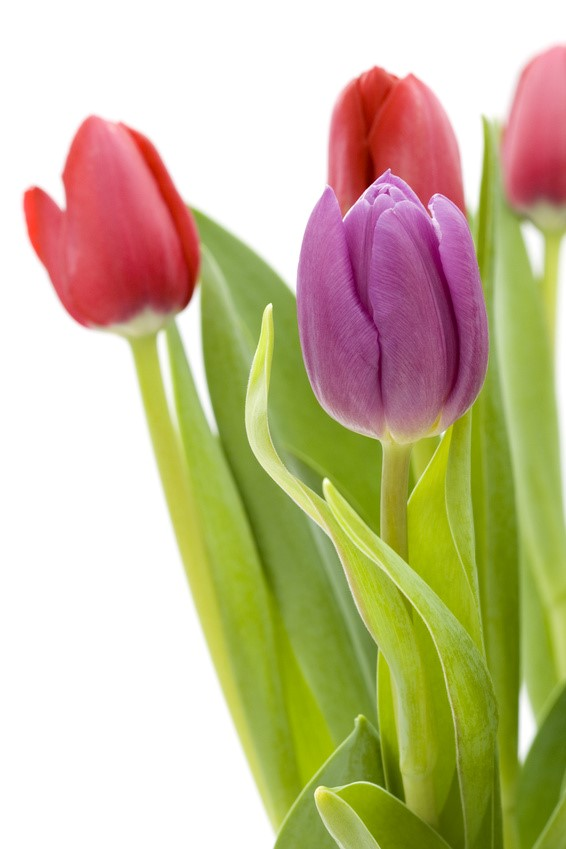
\includegraphics[width=0.3\textwidth]{tulipany}
		\caption{Tulipány před ozářením kryptonitem. Fotografie: autor.}
	\end{center}
\end{figure}
 
 
Obrázky číslujte podle hlavní kapitoly, ve které se vyskytují. Podkapitoly se již neuvažují. 
To znamená, že obrázky v úvodu (typicky kap. 1) budou: Obr.~1.1, Obr.~1.2 atd. V metodách (typicky druhá velká kapitola) budou číslovány Obr.~2.1, Obr.~2.2, Obr.~2.3 atd. 
Podrobněji viz dokument Často kladené dotazy týkající se psaní diplomové práce, dostupný na:
\url{https://predmety.fbmi.cvut.cz/cs/17pmbds2}

Popis tabulky, na rozdíl od obrázku, je zpravidla nad tabulkou, viz Tabulka \ref{tab:tabulka}. 
Není nutné v něm opisovat celý obsah záhlaví tabulky, které následuje hned vzápětí. 
Jednotlivé proměnné v tabulce jsou řazeny do sloupců. 
V tabulce jsou nezávislé proměnné, kategorie probandů apod. řazeny vlevo, závislé proměnné vpravo. 
Jednotky uvádějte v kulatých závorkách v záhlaví tabulky, ne u každého čísla zvlášť. 
Vysvětlující poznámky (např. dosažená hladina významnosti, zda jsou data udávána jako průměr a směrodatná chyba průměru, jaký statistický test byl použit apod.) jsou umisťovány pod tabulku a odkaz na ně se udává jako horní index (symboly, čísla, písmena) na příslušném místě tabulky. 
Na každý obrázek a tabulku je třeba odkazovat z hlavního textu.

\begin{table}[h]
	\label{tab:tabulka}
	\catcode`\-=12          % Tento řádek je tam kvůli použití cline pro czech babel. Jinak to bere pomlčku jako znak a nevnímá ji jako rozsah. 
	\begin{center}
	\begin{threeparttable}      % Pokud nepotřebujete vysvětlení pod tabulkou, stačí použít tabular (vypustit threeparttable a tablenotes).
		\caption[Tady může být kratší popisek pro seznam tabulek.]{Reakční čas $T_{20}$ signálu periferní saturace kyslíkem, $Sp$O$_2$, měřený třemi různými přístroji.}
		\vspace{1ex}
		\begin{tabular}{lccc}
			\noalign{\hrule height 2pt}
			                & \multicolumn{3}{c}{$T_{20}(s)$}                           \\  \cline{2-4}
			Fáze            & Root Radical-7    & Nellcor N-600     & Carescape B650    \\ \hline
			Hypoxická	    & $52\pm15^{*}$	    & $65\pm19^{*}$     & $56\pm15$         \\
            Hyperoxická	    & $43\pm14$	        & $55\pm28$	        & $49\pm15$         \\
            Hyperkapnická	& $75\pm23$	        & $119\pm47^{\sharp}$	& $73\pm41^{\sharp}$  \\   \noalign{\hrule height 2pt}
	    \end{tabular}
	    \begin{tablenotes}
            %\small
            \item Data byla měřena pro shodnou skupinu 14 probandů a jsou uvedena jako aritmetický průměr $\pm$ směrodatná odchylka. Symboly $^{*}$ a $^{\sharp}$ značí statisticky významný rozdíl $ \left( p \leq 0,05 \right) $ časů pro shodnou fázi.
            \end{tablenotes}
	\end{threeparttable}
	\end{center}
\end{table}


